\documentclass{standalone}
\usepackage{tikz}
\usetikzlibrary{patterns, positioning}


\begin{document}
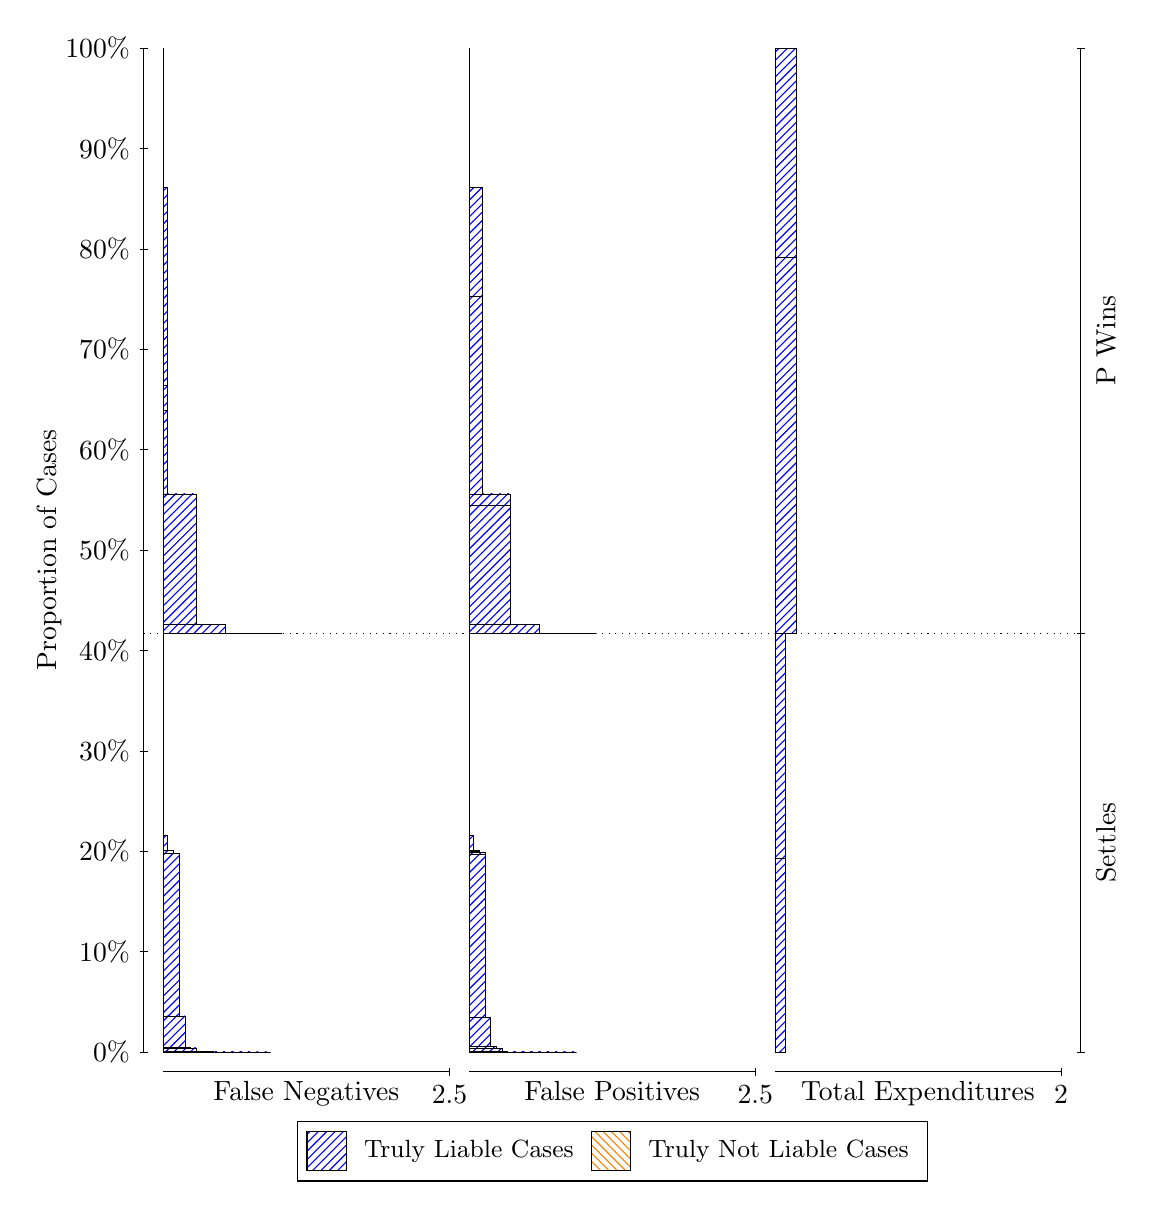
\begin{tikzpicture}
\draw[black, very thin] (1.5,1.75) -- (1.5,14.5);
\node[rotate=90, text=black, anchor=center] at (0.3, 8.125) {Proportion of Cases};
\draw[black, very thin] (1.45,1.75) -- (1.55,1.75);
\node[text=black, anchor=east] at (1.45, 1.75) {0\%};
\draw[black, very thin] (1.45,3.025) -- (1.55,3.025);
\node[text=black, anchor=east] at (1.45, 3.025) {10\%};
\draw[black, very thin] (1.45,4.3) -- (1.55,4.3);
\node[text=black, anchor=east] at (1.45, 4.3) {20\%};
\draw[black, very thin] (1.45,5.575) -- (1.55,5.575);
\node[text=black, anchor=east] at (1.45, 5.575) {30\%};
\draw[black, very thin] (1.45,6.85) -- (1.55,6.85);
\node[text=black, anchor=east] at (1.45, 6.85) {40\%};
\draw[black, very thin] (1.45,8.125) -- (1.55,8.125);
\node[text=black, anchor=east] at (1.45, 8.125) {50\%};
\draw[black, very thin] (1.45,9.4) -- (1.55,9.4);
\node[text=black, anchor=east] at (1.45, 9.4) {60\%};
\draw[black, very thin] (1.45,10.675) -- (1.55,10.675);
\node[text=black, anchor=east] at (1.45, 10.675) {70\%};
\draw[black, very thin] (1.45,11.95) -- (1.55,11.95);
\node[text=black, anchor=east] at (1.45, 11.95) {80\%};
\draw[black, very thin] (1.45,13.225) -- (1.55,13.225);
\node[text=black, anchor=east] at (1.45, 13.225) {90\%};
\draw[black, very thin] (1.45,14.5) -- (1.55,14.5);
\node[text=black, anchor=east] at (1.45, 14.5) {100\%};

\draw[black, very thin] (13.4,1.75) -- (13.4,14.5);
\draw[black, very thin] (13.35,1.75) -- (13.45,1.75);
\node[anchor=west] at (13.35, 1.75) {};
\draw[black, very thin] (13.35,7.0653) -- (13.45,7.0653);
\node[anchor=west] at (13.35, 7.0653) {};
\draw[black, very thin] (13.35,14.5) -- (13.45,14.5);
\node[anchor=west] at (13.35, 14.5) {};

\draw[black, very thin, pattern color=blue, pattern=north east lines] (1.75,1.75) rectangle (3.1125,1.75);
\draw[black, very thin, pattern color=blue, pattern=north east lines] (1.75,1.75) rectangle (2.8218,1.75);
\draw[black, very thin, pattern color=blue, pattern=north east lines] (1.75,1.75) rectangle (2.7492,1.75);
\draw[black, very thin, pattern color=blue, pattern=north east lines] (1.75,1.75) rectangle (2.6765,1.75);
\draw[black, very thin, pattern color=blue, pattern=north east lines] (1.75,1.75) rectangle (2.5312,1.7501);
\draw[black, very thin, pattern color=blue, pattern=north east lines] (1.75,1.7501) rectangle (2.4585,1.7501);
\draw[black, very thin, pattern color=blue, pattern=north east lines] (1.75,1.7501) rectangle (2.3858,1.7526);
\draw[black, very thin, pattern color=blue, pattern=north east lines] (1.75,1.7526) rectangle (2.3132,1.7526);
\draw[black, very thin, pattern color=blue, pattern=north east lines] (1.75,1.7526) rectangle (2.2405,1.7536);
\draw[black, very thin, pattern color=blue, pattern=north east lines] (1.75,1.7536) rectangle (2.1678,1.8029);
\draw[black, very thin, pattern color=blue, pattern=north east lines] (1.75,1.8029) rectangle (2.0952,1.8038);
\draw[black, very thin, pattern color=blue, pattern=north east lines] (1.75,1.8038) rectangle (2.0952,1.8047);
\draw[black, very thin, pattern color=blue, pattern=north east lines] (1.75,1.8047) rectangle (2.0225,2.2078);
\draw[black, very thin, pattern color=blue, pattern=north east lines] (1.75,2.2078) rectangle (1.9498,2.2079);
\draw[black, very thin, pattern color=blue, pattern=north east lines] (1.75,2.2079) rectangle (1.9498,4.2751);
\draw[black, very thin, pattern color=blue, pattern=north east lines] (1.75,4.2751) rectangle (1.8772,4.3099);
\draw[black, very thin, pattern color=blue, pattern=north east lines] (1.75,4.3099) rectangle (1.8045,4.5015);
\draw[black, very thin, pattern color=orange, pattern=north west lines] (1.75,4.5015) rectangle (1.75,4.5015);
\draw[black, very thin, pattern color=blue, pattern=north east lines] (1.75,4.5015) rectangle (1.75,7.0653);
\draw[black, very thin, pattern color=blue, pattern=north east lines] (1.75,7.0653) rectangle (3.2578,7.0653);
\draw[black, very thin, pattern color=blue, pattern=north east lines] (1.75,7.0653) rectangle (2.8945,7.0665);
\draw[black, very thin, pattern color=blue, pattern=north east lines] (1.75,7.0665) rectangle (2.5312,7.1795);
\draw[black, very thin, pattern color=blue, pattern=north east lines] (1.75,7.1795) rectangle (2.1678,8.8372);
\draw[black, very thin, pattern color=blue, pattern=north east lines] (1.75,8.8372) rectangle (1.8045,9.9016);
\draw[black, very thin, pattern color=blue, pattern=north east lines] (1.75,9.9016) rectangle (1.8045,10.22);
\draw[black, very thin, pattern color=blue, pattern=north east lines] (1.75,10.22) rectangle (1.8045,12.727);
\draw[black, very thin, pattern color=orange, pattern=north west lines] (1.75,12.727) rectangle (1.75,12.727);
\draw[black, very thin, pattern color=blue, pattern=north east lines] (1.75,12.727) rectangle (1.75,14.5);
\draw[black, very thin, pattern color=orange, pattern=north west lines] (5.6333,1.75) rectangle (6.9958,1.75);
\draw[black, very thin, pattern color=blue, pattern=north east lines] (5.6333,1.75) rectangle (6.9958,1.75);
\draw[black, very thin, pattern color=orange, pattern=north west lines] (5.6333,1.75) rectangle (6.8505,1.75);
\draw[black, very thin, pattern color=blue, pattern=north east lines] (5.6333,1.75) rectangle (6.8505,1.75);
\draw[black, very thin, pattern color=orange, pattern=north west lines] (5.6333,1.75) rectangle (6.7052,1.75);
\draw[black, very thin, pattern color=blue, pattern=north east lines] (5.6333,1.75) rectangle (6.7052,1.75);
\draw[black, very thin, pattern color=blue, pattern=north east lines] (5.6333,1.75) rectangle (6.6325,1.75);
\draw[black, very thin, pattern color=orange, pattern=north west lines] (5.6333,1.75) rectangle (6.5598,1.75);
\draw[black, very thin, pattern color=blue, pattern=north east lines] (5.6333,1.75) rectangle (6.5598,1.75);
\draw[black, very thin, pattern color=blue, pattern=north east lines] (5.6333,1.75) rectangle (6.4872,1.75);
\draw[black, very thin, pattern color=orange, pattern=north west lines] (5.6333,1.75) rectangle (6.4145,1.75);
\draw[black, very thin, pattern color=blue, pattern=north east lines] (5.6333,1.75) rectangle (6.4145,1.7501);
\draw[black, very thin, pattern color=blue, pattern=north east lines] (5.6333,1.7501) rectangle (6.3418,1.7503);
\draw[black, very thin, pattern color=blue, pattern=north east lines] (5.6333,1.7503) rectangle (6.2692,1.7519);
\draw[black, very thin, pattern color=orange, pattern=north west lines] (5.6333,1.7519) rectangle (6.2692,1.7519);
\draw[black, very thin, pattern color=blue, pattern=north east lines] (5.6333,1.7519) rectangle (6.2692,1.7519);
\draw[black, very thin, pattern color=blue, pattern=north east lines] (5.6333,1.7519) rectangle (6.1965,1.7523);
\draw[black, very thin, pattern color=blue, pattern=north east lines] (5.6333,1.7523) rectangle (6.1238,1.753);
\draw[black, very thin, pattern color=orange, pattern=north west lines] (5.6333,1.753) rectangle (6.1238,1.753);
\draw[black, very thin, pattern color=blue, pattern=north east lines] (5.6333,1.753) rectangle (6.1238,1.7539);
\draw[black, very thin, pattern color=blue, pattern=north east lines] (5.6333,1.7539) rectangle (6.0512,1.8004);
\draw[black, very thin, pattern color=blue, pattern=north east lines] (5.6333,1.8004) rectangle (5.9785,1.8207);
\draw[black, very thin, pattern color=blue, pattern=north east lines] (5.6333,1.8207) rectangle (5.9058,2.1866);
\draw[black, very thin, pattern color=blue, pattern=north east lines] (5.6333,2.1866) rectangle (5.9058,2.1868);
\draw[black, very thin, pattern color=orange, pattern=north west lines] (5.6333,2.1868) rectangle (5.8332,2.1868);
\draw[black, very thin, pattern color=blue, pattern=north east lines] (5.6333,2.1868) rectangle (5.8332,4.2551);
\draw[black, very thin, pattern color=blue, pattern=north east lines] (5.6333,4.2551) rectangle (5.8332,4.2806);
\draw[black, very thin, pattern color=blue, pattern=north east lines] (5.6333,4.2806) rectangle (5.7605,4.2977);
\draw[black, very thin, pattern color=blue, pattern=north east lines] (5.6333,4.2977) rectangle (5.7605,4.3138);
\draw[black, very thin, pattern color=blue, pattern=north east lines] (5.6333,4.3138) rectangle (5.6878,4.5054);
\draw[black, very thin, pattern color=blue, pattern=north east lines] (5.6333,4.5054) rectangle (5.6333,7.0653);
\draw[black, very thin, pattern color=orange, pattern=north west lines] (5.6333,7.0653) rectangle (7.2502,7.0653);
\draw[black, very thin, pattern color=blue, pattern=north east lines] (5.6333,7.0653) rectangle (7.2502,7.0653);
\draw[black, very thin, pattern color=orange, pattern=north west lines] (5.6333,7.0653) rectangle (6.8868,7.0653);
\draw[black, very thin, pattern color=blue, pattern=north east lines] (5.6333,7.0653) rectangle (6.8868,7.0665);
\draw[black, very thin, pattern color=orange, pattern=north west lines] (5.6333,7.0665) rectangle (6.5235,7.0665);
\draw[black, very thin, pattern color=blue, pattern=north east lines] (5.6333,7.0665) rectangle (6.5235,7.1804);
\draw[black, very thin, pattern color=blue, pattern=north east lines] (5.6333,7.1804) rectangle (6.1602,8.6903);
\draw[black, very thin, pattern color=orange, pattern=north west lines] (5.6333,8.6903) rectangle (6.1602,8.6903);
\draw[black, very thin, pattern color=blue, pattern=north east lines] (5.6333,8.6903) rectangle (6.1602,8.8381);
\draw[black, very thin, pattern color=blue, pattern=north east lines] (5.6333,8.8381) rectangle (5.7968,11.345);
\draw[black, very thin, pattern color=orange, pattern=north west lines] (5.6333,11.345) rectangle (5.7968,11.345);
\draw[black, very thin, pattern color=blue, pattern=north east lines] (5.6333,11.345) rectangle (5.7968,12.728);
\draw[black, very thin, pattern color=blue, pattern=north east lines] (5.6333,12.728) rectangle (5.6333,14.5);
\draw[black, very thin, pattern color=orange, pattern=north west lines] (9.5167,1.75) rectangle (9.6529,1.75);
\draw[black, very thin, pattern color=blue, pattern=north east lines] (9.5167,1.75) rectangle (9.6529,4.2062);
\draw[black, very thin, pattern color=orange, pattern=north west lines] (9.5167,4.2062) rectangle (9.6529,4.2062);
\draw[black, very thin, pattern color=blue, pattern=north east lines] (9.5167,4.2062) rectangle (9.6529,7.0653);
\draw[black, very thin, pattern color=orange, pattern=north west lines] (9.5167,7.0653) rectangle (9.7892,7.0653);
\draw[black, very thin, pattern color=blue, pattern=north east lines] (9.5167,7.0653) rectangle (9.7892,11.845);
\draw[black, very thin, pattern color=orange, pattern=north west lines] (9.5167,11.845) rectangle (9.7892,11.845);
\draw[black, very thin, pattern color=blue, pattern=north east lines] (9.5167,11.845) rectangle (9.7892,14.5);
\draw[black, dotted] (1.5,7.0653) -- (13.4,7.0653);
\draw[black, very thin] (1.75,1.5) -- (5.3833,1.5);
\node[text=black, anchor=north] at (3.5667, 1.5) {False Negatives};
\draw[black, very thin] (5.3833,1.45) -- (5.3833,1.55);
\node[text=black, anchor=north] at (5.3833, 1.45) {2.5};

\draw[black, very thin] (5.6333,1.5) -- (9.2667,1.5);
\node[text=black, anchor=north] at (7.45, 1.5) {False Positives};
\draw[black, very thin] (9.2667,1.45) -- (9.2667,1.55);
\node[text=black, anchor=north] at (9.2667, 1.45) {2.5};

\draw[black, very thin] (9.5167,1.5) -- (13.15,1.5);
\node[text=black, anchor=north] at (11.333, 1.5) {Total Expenditures};
\draw[black, very thin] (13.15,1.45) -- (13.15,1.55);
\node[text=black, anchor=north] at (13.15, 1.45) {2};

\node[text=black, centered, rotate=90] at (13.72, 4.4076) {Settles};
\node[text=black, centered, rotate=90] at (13.72, 10.783) {P Wins};

\draw (7.449999999999999,1.5) node[draw=none] (baseCoordinate) {};
\begin{scope}[align=center]
        \matrix[scale=0.5, draw=black, below=0.5cm of baseCoordinate, nodes={draw}, column sep=0.1cm]{
            \node[rectangle, draw, minimum width=0.5cm, minimum height=0.5cm, pattern color=blue, pattern=north east lines] {}; &
            \node[draw=none, font=\small, text=black] (B) {Truly Liable Cases}; &
            \node[rectangle, draw, minimum width=0.5cm, minimum height=0.5cm, pattern color=orange, pattern=north west lines] {}; &
            \node[draw=none, font=\small, text=black] (B) {Truly Not Liable Cases}; \\
            };
\end{scope}

\end{tikzpicture}
\end{document}